\documentclass[conference]{IEEEtran}
\IEEEoverridecommandlockouts

\usepackage[utf8]{inputenc}
\usepackage[T1]{fontenc}
\usepackage{graphicx}
\usepackage{booktabs}
\usepackage{url}
\usepackage{amsmath}

\hyphenation{report historical laporan historis}

\title{Aegis: Crowdfunding Berbasis Milestone di Ethereum dengan Voting Berbobot Kontribusi}

\author{\IEEEauthorblockN{Rifqi Ramadhan, George Wiliam Thomas Gonata, Samuel Tanaka Sibarani, dan Riri Fitri Sari}
\IEEEauthorblockA{Departemen Teknik Elektro, Fakultas Teknik, Universitas Indonesia\\
Email: {\tiny \texttt{rifqi.ramadhan22@ui.ac.id}, \texttt{george.william@ui.ac.id},}\\
{\tiny \texttt{samuel.tanaka@ui.ac.id}, \texttt{riri@ui.ac.id}}}}

\begin{document}
\maketitle

\begin{abstract}
Aegis, a blockchain-enabled decentralized crowdfunding concept to be built on the work of Ethereum, introduced post-campaign accountability through contribution-weighted voting on project milestones. Unlike traditional centralized crowdfunding platforms that release funds in bulk immediately after a campaign ends, Aegis locks the raised capital in a project-specific smart contract escrow. The funds are then conditionally released to the creator in tranches, each corresponding to a specific project milestone. Creators must submit detailed progress reports (stored as metadata), which backers review and vote upon. Backers' voting weights are proportional to their financial exposure (ETH contribution). If a milestone report is approved by a majority, the allocated tranche is released; if rejected, or if the project is cancelled, backers can claim proportional refunds from the remaining contract balance. We implement the core contracts (Factory and Project) and a React-based frontend application integrated with MetaMask. The results show that the platform successfully maintains correctness in state transitions and refund processes on a local Hardhat network, as verified through comparison with the industry-standard Juicebox Protocol and academic hybrid blockchain-AI architectures.
\end{abstract}
\renewcommand{\abstractname}{Abstrak}
\begin{abstract}
Aegis, sebuah konsep crowdfunding terdesentralisasi berbasis blockchain yang dibangun di atas karya Ethereum, memperkenalkan akuntabilitas pasca-kampanye melalui voting berbobot kontribusi pada milestone proyek. Berbeda dengan platform crowdfunding terpusat tradisional yang mencairkan dana secara penuh segera setelah kampanye berakhir, Aegis mengunci modal yang terkumpul dalam escrow smart contract khusus proyek. Dana tersebut kemudian dicairkan secara bersyarat kepada kreator dalam bentuk tranche, yang masing-masing sesuai dengan milestone proyek tertentu. Kreator harus mengirimkan laporan kemajuan terperinci (disimpan sebagai metadata), yang ditinjau dan divalidasi oleh para backer. Bobot voting backer sebanding dengan eksposur finansial mereka (kontribusi ETH). Jika laporan milestone disetujui oleh mayoritas, tranche yang dialokasikan akan dicairkan; jika ditolak, atau jika proyek dibatalkan, backer dapat mengklaim pengembalian dana (refund) proporsional dari sisa saldo kontrak. Kami mengimplementasikan contract inti (Factory dan Project) dan aplikasi frontend berbasis React yang terhubung melalui MetaMask. Hasil evaluasi menunjukkan bahwa platform ini berhasil mempertahankan kebenaran dalam transisi status dan proses refund pada jaringan Hardhat lokal, seperti yang diverifikasi melalui perbandingan dengan Juicebox Protocol standar industri dan arsitektur crowdfunding hybrid blockchain-AI akademis.
\end{abstract}

\begin{IEEEkeywords}
Blockchain, Crowdfunding, Smart Contract, Ethereum, Pendanaan Milestone, Web3, Voting Berbobot Kontribusi
\end{IEEEkeywords}

\section{Pendahuluan}

\subsection{Definisi Masalah}
Crowdfunding telah berkembang sebagai mekanisme yang kuat untuk mendemokratisasi penggalangan modal, memungkinkan kreator mendanai proyek melalui kontribusi kecil dari basis pendukung (backer) global. Namun, platform terpusat tradisional (seperti Kickstarter dan GoFundMe) menghadapi keterbatasan serius dalam hal transparansi, tata kelola dana, dan akuntabilitas pasca-kampanye. Setelah proyek berhasil memenuhi tujuan pendanaannya, akumulasi modal biasanya ditransfer secara penuh (*bulk release*) kepada kreator. Para backer dibiarkan tanpa kontrol atas bagaimana dana tersebut dibelanjakan, sehingga penyelewengan dana atau pengabaian proyek pasca-kampanye sering terjadi. Ini menciptakan masalah agensi (*principal-agent problem*) klasik di mana insentif kreator (agen) menyimpang dari kepentingan backer (prinsipal) segera setelah fase pendanaan selesai.

\subsection{Analisis Kebutuhan Blockchain}
Untuk mengatasi tantangan ini, diperlukan pendekatan terdesentralisasi menggunakan teknologi blockchain dan smart contract. Blockchain sangat cocok untuk memecahkan masalah ketiadaan kepercayaan dalam crowdfunding karena karakteristik berikut:
\begin{itemize}
	\item \textbf{Decentralized Escrow}: Smart contract dapat bertindak sebagai pihak ketiga yang netral dan dikendalikan secara terprogram untuk mengunci kontribusi tanpa bergantung pada perantara terpusat.
	\item \textbf{Immutability dan Auditability}: Setiap kontribusi, pengiriman laporan milestone, dan suara voting dicatat secara permanen on-chain, menyediakan riwayat transaksi transparan yang mencegah manipulasi historis.
	\item \textbf{Automated Rule Execution}: Aturan yang mengatur pelepasan dana, periode voting, dan pengembalian dana dieksekusi secara deterministik dan terprogram, menghilangkan bias manusia atau intervensi platform terpusat.
\end{itemize}
Meskipun demikian, sekadar memindahkan model crowdfunding tradisional ke blockchain tidak menyelesaikan masalah agensi pasca-kampanye. Kreator masih dapat menarik semua dana dan mengabaikan proyek. Oleh karena itu, teknologi blockchain merupakan fondasi yang diperlukan (*necessary*) tetapi belum cukup (*not sufficient*); ia harus dipadukan dengan mekanisme penegakan berbasis milestone.

\subsection{Inovasi Aegis}
Paper ini menyajikan Aegis, sebuah konsep platform crowdfunding terdesentralisasi yang dirancang untuk menjembatani celah kepercayaan pasca-kampanye. Inovasi utama Aegis terletak pada integrasi escrow terikat milestone dengan model voting berbobot kontribusi.

Sebelum memulai kampanye, kreator proyek harus menentukan serangkaian milestone terstruktur dengan tranche pendanaan terkait. Dana kontribusi dalam bentuk Ether (ETH) dikunci dengan aman di smart contract proyek. Untuk membuka setiap tranche, kreator wajib mengirimkan laporan kemajuan yang berisi bukti kerja. Backer kemudian memberikan suara untuk menyetujui atau menolak laporan tersebut, dengan bobot suara ditentukan oleh jumlah kontribusi masing-masing. Hal ini menyelaraskan hak suara langsung dengan risiko finansial backer, memitigasi serangan Sybil, dan memastikan otoritas pengambilan keputusan sebanding dengan eksposur modal.

Kontribusi utama dari paper ini diringkas sebagai berikut:
\begin{itemize}
	\item Model voting berbobot kontribusi yang menyelaraskan kekuatan suara dengan risiko finansial backer sekaligus memberikan ketahanan terhadap serangan Sybil.
	\item Arsitektur aplikasi terdesentralisasi (DApp) end-to-end yang mencakup kontrak proyek yang dideploy melalui factory serta antarmuka pengguna React yang terhubung dengan MetaMask.
	\item Model state machine ketat yang mengatur siklus hidup proyek (Funding, Active, Completed, Cancelled) untuk mencegah transisi status yang tidak valid.
	\item Analisis komparatif Aegis terhadap Juicebox Protocol komersial dan arsitektur hybrid blockchain-AI akademis.
\end{itemize}

Sisa dari paper ini disusun sebagai berikut: Section II meninjau penelitian terkait. Section III menjelaskan metodologi voting berbobot kontribusi yang diusulkan. Section IV merinci desain dan arsitektur sistem. Section V menyajikan detail implementasi sistem. Section VI mengevaluasi konsep platform melalui skenario pengujian dan membahas batasan sistem. Akhirnya, Section VII menyimpulkan paper ini dan menguraikan penelitian masa depan.

\section{Tinjauan Pustaka}

\subsection{Juicebox Protocol (Industri Komersial)}
The Juicebox Protocol is a widely used decentralized treasury management and crowdfunding platform on Ethereum \cite{juicebox}. It allows communities to configure funding cycles, issue tokens, and manage treasury redemptions. Juicebox sangat fleksibel dan terukur (scalable) untuk crowdfunding dan blockchain DAO karena mengotomatiskan penerbitan token, pembayaran kas, dan alokasi multi-tujuan dalam siklus pendanaan yang dapat dikonfigurasi, sehingga mengurangi overhead operasional. Namun, fokus utamanya adalah pada pendanaan berkelanjutan dan tokenomika, bukan pada penegakan milestone terstruktur. Di Juicebox, pelepasan dana umumnya diatur oleh konfigurasi siklus tetap atau alokasi multisig terbuka. Tidak ada mekanisme bawaan langsung yang mengikat tranche dana dengan laporan milestone yang ditinjau backer, sehingga membatasi penerapannya untuk proyek yang membutuhkan akuntabilitas bertahap yang ketat.

\subsection{Sistem Crowdfunding Blockchain Akademis}
Dalam literatur akademis, beberapa peneliti telah mengusulkan penggunaan smart contract berbasis Ethereum untuk meningkatkan kepercayaan dan memitigasi fraud dalam crowdfunding. Rathore dan Rizvi \cite{rathore2023decentralized} mengeksplorasi platform crowdfunding terdesentralisasi dasar pada blockchain, menyoroti keuntungan smart contract dalam menghapus perantara terpusat dan mengurangi biaya transaksi. Serupa dengan itu, Jayapal, Xavier, and Arunachalam \cite{jayapal2023capitalizing} memeriksa efisiensi smart contract Ethereum dalam mengotomatisasi alur kerja kampanye, memastikan kreator menerima dana hanya jika target terpenuhi, sehingga mengurangi risiko finansial bagi backer.

Untuk mengatasi asimetri informasi, Ahmad dan Rahman \cite{ahmad2021applying} mengusulkan penerapan smart contract untuk meningkatkan kepercayaan dengan menjaga transparansi penuh pada transaksi dan status proyek. Aprialim, Adnan, dan Paundu \cite{aprialim2021penerapan} menyajikan model integrasi smart contract yang berfokus pada keamanan struktural selama fase pendanaan. Lebih lanjut, BitFund \cite{bitfund2020} memodelkan kerangka kerja crowdfunding terbuka yang dirancang untuk kota cerdas, menekankan audit buku besar publik.

Namun, model-model ini terutama berfokus pada fase pra-kampanye dan kampanye aktif, membiarkan fase pasca-kampanye tidak terkelola. Setelah tujuan pendanaan terpenuhi, arsitektur ini langsung mencairkan seluruh dana, sehingga gagal menyelesaikan masalah pengabaian proyek pasca-kampanaan.

\subsection{Model Escrow dan Tata Kelola Terdesentralisasi}
Untuk melindungi dana pasca-kampanye, beberapa sistem menggabungkan struktur escrow dan tata kelola. Shelke dkk. \cite{shelke2022blockchain} mengusulkan kerangka kerja escrow terdesentralisasi yang mengunci kontribusi dan memungkinkan intervensi manual oleh backer, meskipun tidak memiliki alur kerja milestone terstruktur. Zichichi dkk. \cite{zichichi2019likestarter} mengembangkan LikeStarter, DAO sosial berbasis smart contract yang menggunakan bukti sosial dan voting untuk menyelaraskan struktur insentif antara kreator dan backer.

Pembayaran milestone berkala secara formal dimodelkan oleh Alruwaili dan Kruger \cite{alruwaili2020milestone}, yang mengusulkan pemanfaatan sistem e-voting yang adil untuk menyetujui tranche secara berurutan. Meskipun model mereka kuat secara matematis, model tersebut bergantung pada skema voting kriptografi kompleks yang sulit dideploy on-chain karena kendala biaya gas. Aegis menyederhanakan hal ini dengan menerapkan sistem voting mayoritas sederhana berbobot kontribusi langsung di dalam kontrak proyek, yang efisien dalam penggunaan gas dan mudah diintegrasikan dengan antarmuka Web3 standar.

Untuk memvalidasi keamanan alur kerja yang kompleks ini, Villanueva, Srinivasan, dan Rehman \cite{villanueva2025metamorphic} mengusulkan teknik pengujian metamorfik untuk mendeteksi potensi kerentanan logis dalam kontrak crowdfunding berbasis Ethereum. Chen dkk. \cite{chen2023dcc} membahas model tata kelola bersama terdesentralisasi untuk meningkatkan keberlanjutan proyek jangka panjang, menekankan pentingnya pengawasan kolaboratif.

Tabel~\ref{tab:comparison} menyoroti perbedaan utama antara Aegis dan solusi terkait lainnya, menunjukkan bahwa Aegis menempati posisi unik dengan menyediakan DApp praktis yang end-to-end dengan voting milestone berbobot kontribusi yang kuat, yang dapat diperluas ke kasus penggunaan lain seperti distribusi hibah terdesentralisasi (decentralized grants), pendanaan barang publik (public goods funding), dan verifikasi kesepakatan tingkat layanan (SLA).

\begin{table}[t]
\centering
\caption{Perbandingan Aegis dengan Solusi Terkait}
\label{tab:comparison}
\begin{tabular}{lccc}
\toprule
\textbf{Kriteria} & \textbf{Juicebox \cite{juicebox}} & \textbf{Hybrid AI \cite{hybridai}} & \textbf{Aegis} \\
\midrule
Berbasis Ethereum & Ya & Ya & Ya \\
Manajemen Milestone & Terbatas & Ya & Ya \\
Voting Komunitas & Terbatas & Terbatas & Ya \\
Pelepasan Dana Otomatis & Sebagian & Ya & Ya \\
Verifikasi AI & Tidak & Ya & Tidak \\
DApp End-to-End & Ya & Tidak & Ya \\
\bottomrule
\end{tabular}
\end{table}

\section{Metodologi yang Diusulkan}
Aegis mengatasi risiko pasca-kampanye melalui mekanisme voting milestone berbobot kontribusi yang baru. Persyaratan sistem dan dinamika voting diformalkan di bawah ini.

\subsection{Model Voting Berbobot Kontribusi}
Misalkan $P$ adalah proyek crowdfunding dengan target pendanaan total $G$ dan himpunan backer $B = \{1, 2, \dots, n\}$. Setiap backer $i \in B$ memberikan kontribusi Ether $c_i > 0$ sedemikian rupa sehingga jumlah dana terkumpul $C_{\text{total}}$ memenuhi:
\begin{equation}
C_{\text{total}} = \sum_{i=1}^{n} c_i \ge G
\end{equation}
Sebuah proyek terstruktur menjadi serangkaian milestone berurutan $M = \{M_1, M_2, \dots, M_m\}$, di mana setiap milestone $M_j$ memiliki tranche pendanaan yang dialokasikan $A_j > 0$ sedemikian rupa sehingga:
\begin{equation}
\sum_{j=1}^{m} A_j = G
\end{equation}

Ketika kreator mengirimkan bukti kemajuan untuk milestone $M_j$, backer dapat memberikan suara $v_{i,j} \in \{\text{Setuju}, \text{Tolak}\}$. Bobot voting $w_i$ dari backer $i$ didefinisikan sebagai kontribusi finansial mereka:
\begin{equation}
w_i = c_i
\end{equation}
Misalkan $V_Y$ adalah jumlah bobot dari para backer yang memilih setuju, dan $V_N$ adalah jumlah bobot dari para backer yang memilih tolak:
\begin{equation}
V_Y = \sum_{i \in B, v_{i,j} = \text{Setuju}} w_i, \quad V_N = \sum_{i \in B, v_{i,j} = \text{Tolak}} w_i
\end{equation}
Milestone $M_j$ disetujui jika bobot persetujuan mencapai mayoritas sederhana dari total pendanaan proyek:
\begin{equation}
V_Y > \frac{C_{\text{total}}}{2}
\end{equation}
Setelah disetujui, tranche $A_j$ dicairkan ke dompet kreator. Jika $V_N > C_{\text{total}}/2$, milestone ditolak, yang menghentikan proyek dan memungkinkan backer untuk mengklaim pengembalian dana.

\subsection{Diskusi Desain Voting dan Resistensi Sybil}
Pilihan model voting berbobot kontribusi mengatasi beberapa tantangan penting dalam tata kelola terdesentralisasi:
\begin{itemize}
	\item \textbf{Mitigasi Serangan Sybil}: Sistem blockchain standar yang menerapkan aturan satu-alamat-satu-suara sangat rentan terhadap serangan Sybil, di mana satu individu membuat banyak alamat Ethereum untuk memanipulasi hasil. Dengan mengikat kekuatan voting langsung ke ETH yang dikontribusikan ($w_i = c_i$), Aegis memastikan bahwa bobot suara terikat pada modal yang terkunci di dalam kontrak, sehingga membuat serangan Sybil menjadi tidak efektif.
	\item \textbf{Penyelarasan Insentif}: Menghubungkan bobot suara dengan kontribusi menyelaraskan otoritas pengambilan keputusan dengan risiko finansial. Backer yang mendanai porsi lebih besar dari target proyek memikul risiko finansial lebih tinggi dan dengan demikian memiliki hak suara yang lebih besar dalam validasi kemajuan.
	\item \textbf{Penyelesaian Instan vs. Timeout}: Untuk mengoptimalkan efisiensi operasional, kontrak mengevaluasi konsensus secara dinamis pada setiap pengiriman suara. Jika total suara setuju ($V_Y$) atau suara tolak ($V_N$) melebihi ambang batas mayoritas mutlak ($C_{\text{total}}/2$), proses voting diselesaikan secara instan, dan dana dicairkan atau dibekukan. Jika tidak ada mayoritas yang dicapai, voting tetap terbuka hingga berakhirnya periode voting ($T_{\text{voting}} = 7$ hari), setelah itu status milestone ditentukan berdasarkan akumulasi mayoritas sederhana.
\end{itemize}

\subsection{Mekanisme Pengembalian Dana (Refund)}
Jika proyek dibatalkan oleh kreator, atau jika milestone ditolak oleh backer, proyek beralih ke status \textit{Cancelled}. Backer berhak mengklaim pengembalian dana yang proporsional dengan kontribusi mereka dari sisa saldo kontrak $R$. Jumlah refund $R_i$ untuk backer $i$ dihitung sebagai:
\begin{equation}
\label{eq:refund}
R_i = c_i \times \frac{R}{C_{\text{total}} - C_{\text{released}}}
\end{equation}
di mana $C_{\text{released}}$ is jumlah total dana yang telah dicairkan kepada kreator untuk milestone yang disetujui. Rumus ini memastikan bahwa sisa dana escrow yang belum dicairkan dikembalikan kepada backer secara adil, dengan memperhitungkan tranche yang sudah disalurkan untuk pekerjaan yang berhasil diselesaikan.

\section{Desain Sistem}

\subsection{Tinjauan Arsitektur}
Platform Aegis menggunakan topologi terdesentralisasi yang terdiri dari tiga lapisan: Antarmuka Klien (React DApp), Penyedia Web3 (dompet MetaMask), dan Smart Contract Ethereum. Gambar~\ref{fig:usecase} mengilustrasikan diagram use case inti dari platform.

\begin{figure}[h]
\centering
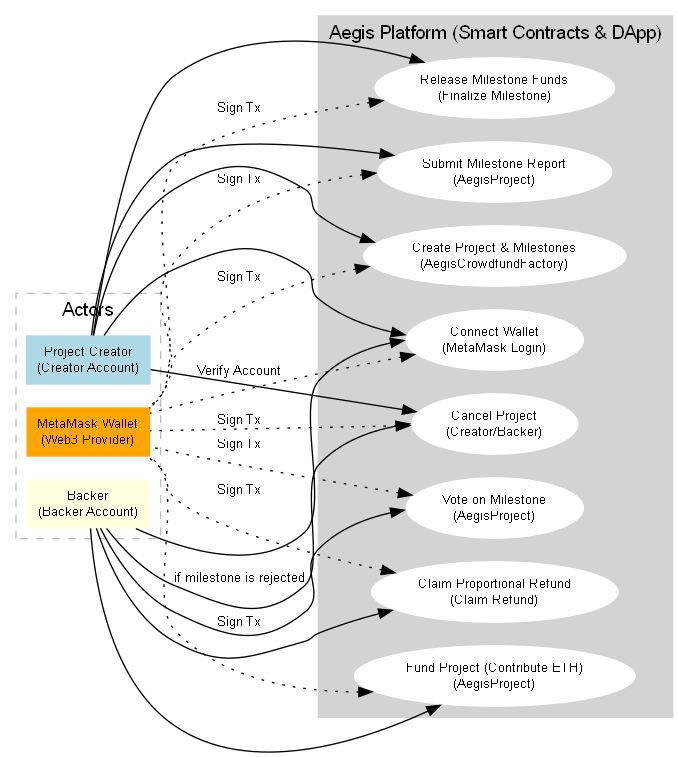
\includegraphics[width=0.75\columnwidth]{../use-case-en.png}
\caption{Diagram use case aktor Aegis dan aksi inti.}
\label{fig:usecase}
\end{figure}

Topologi mengikuti pola factory-project:
\begin{enumerate}
	\item \textbf{AegisCrowdfundFactory}: Kontrak registri tunggal yang dideploy on-chain untuk digunakan kreator dalam meluncurkan kontrak proyek baru secara terstandarisasi. Ini mengurangi overhead gas saat deployment dan menyediakan indeks terpusat dari seluruh kampanye.
	\item \textbf{AegisProject}: Kontrak escrow independen yang dideploy untuk setiap kampanye. Kontrak ini mengelola siklus hidup kampanye, mengamankan kontribusi ETH, mencatat milestone, menangani voting, dan mencairkan dana.
\end{enumerate}

\subsection{Entitas Data dan Mapping}
To enforce governance rules efficiently, the \texttt{AegisProject} smart contract maintains three primary data mapping structures in state storage:
\begin{itemize}
	\item \texttt{contributions (address => uint256)}: Memetakan alamat setiap backer ke jumlah ETH yang mereka kontribusikan. Ini berfungsi sebagai sumber kebenaran untuk pembayaran pengembalian dana dan bobot voting.
	\item \texttt{hasVoted (address => mapping(uint256 => bool))}: Pemetaan bersarang yang melacak apakah backer tertentu telah memberikan suara pada ID milestone tertentu, mencegah voting ganda.
	\item \texttt{milestones (Milestone[])}: Array terurut dari struct `Milestone` yang berisi deskripsi, jumlah dana, status, dan laporan kemajuan.
\end{itemize}

\subsection{Alur Kerja Sistem}
Gambar~\ref{fig:sequence} menggambarkan urutan kronologis interaksi antara pengguna, frontend DApp, MetaMask, dan smart contract selama pelaporan milestone dan voting.

\begin{figure}[h]
\centering
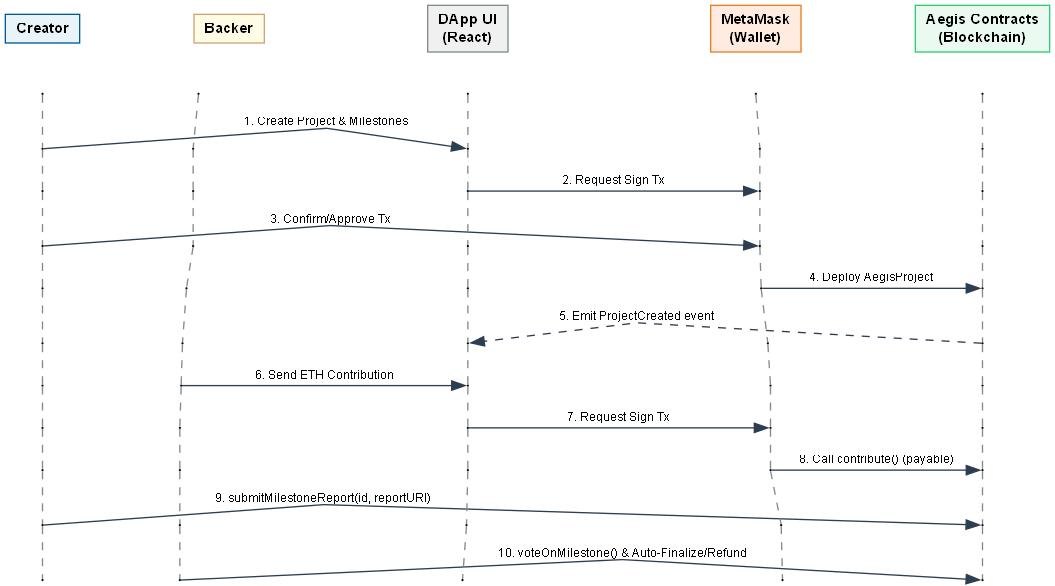
\includegraphics[width=0.9\columnwidth]{../sequence-en.png}
\caption{Sequence diagram interaksi UI-wallet-contract untuk persetujuan milestone.}
\label{fig:sequence}
\end{figure}

Pertama, kreator mengirimkan bukti milestone. Frontend menangkap data ini dan memanggil fungsi `submitMilestoneReport` kontrak, meminta MetaMask untuk menandatangani transaksi. Once confirmed, backers can query the report and cast their vote via `voteOnMilestone`. Kontrak menghitung bobot dan secara otomatis melepaskan tranche jika mayoritas terpenuhi, atau memperbarui status untuk penyelesaian akhir setelah periode voting berakhir.

\subsection{State Machine Siklus Hidup Proyek}
Kontrak `AegisProject` mengimplementasikan state machine yang ketat untuk mencegah serangan reentrancy dan eksekusi di luar urutan. Status didefinisikan sebagai berikut:
\begin{itemize}
	\item \textbf{Funding}: Status awal di mana backer mengirimkan kontribusi ETH. Jika target $G$ tercapai sebelum deadline, status beralih ke \textit{Active}. Jika deadline lewat tanpa memenuhi $G$, proyek beralih ke \textit{Cancelled}, mengaktifkan fitur refund.
	\item \textbf{Active}: Proyek berhasil didanai. Kreator dapat mengirimkan laporan milestone, dan backer melakukan voting.
	\item \textbf{Completed}: Beralih ke status ini secara otomatis ketika semua milestone telah disetujui dan seluruh dana dilepaskan ke kreator.
	\item \textbf{Cancelled}: Dipicu oleh kegagalan pendanaan, pembatalan oleh kreator, atau penolakan milestone oleh voting komunitas. Semua dana yang tersisa dibekukan di escrow, dan backer dapat menarik refund proporsional mereka.
\end{itemize}

\section{Implementasi}
Bagian ini menjelaskan implementasi praktis dari platform Aegis. Basis kode diorganisasikan ke dalam dua lapisan utama: smart contract yang mewakili logika blockchain backend, dan aplikasi frontend terdesentralisasi berbasis React. Proses integrasi komponen-komponen ini bergantung pada penyedia Web3 untuk membangun saluran komunikasi bersama, yang dirinci di bawah ini.

\subsection{Smart Contract Solidity}
Smart contract dikembangkan menggunakan Solidity (v0.8.28) dalam lingkungan Hardhat. Arsitektur dibagi menjadi dua kontrak utama: `AegisCrowdfundFactory.sol` dan `AegisProject.sol`.

\subsubsection{Factory Contract}
`AegisCrowdfundFactory` dideploy sekali dan bertindak sebagai registri pusat. Kontrak ini menyediakan fungsi `createProject(...)` untuk membuat instansiasi kontrak proyek baru on-chain menggunakan kata kunci `new`:
\begin{verbatim}
AegisProject newProject = new AegisProject(
    msg.sender, _name, _description,
    _fundingGoal, _fundingDeadline,
    _mDescriptions, _mAmounts, _mDeadlines
);
projects.push(address(newProject));
\end{verbatim}
Pola ini menciptakan ruang nama terisolasi untuk setiap kampanye crowdfunding, melindungi dana suatu proyek dari masalah teknis di proyek lainnya.

\subsubsection{Project Contract}
Kontrak `AegisProject` berisi variabel status dan logika inti untuk pendanaan serta pelepasan milestone. Kontrak ini menggunakan array struct untuk melacak milestone:
\begin{verbatim}
struct Milestone {
    string description;
    uint256 amount;
    uint256 deadline;
    MilestoneStatus status;
    string reportURI;
    uint256 yesVotes;
    uint256 noVotes;
    uint256 votingDeadline;
}
\end{verbatim}
Di sini, `reportURI` disimpan sebagai string on-chain. Alih-alih mengunggah berkas bukti yang besar secara langsung ke EVM (yang akan memakan biaya gas sangat mahal), frontend React menserialisasi beberapa item bukti ke dalam JSON string ringan dan mengunggahnya ke kontrak.

Untuk mencegah voting ganda, kontrak melacak suara menggunakan pemetaan bersarang:
\begin{verbatim}
mapping(address => mapping(uint256 => bool)) 
    public hasVoted;
\end{verbatim}
Ketika suara dikirimkan, status `hasVoted[voter][milestoneId]` disetel menjadi `true`, dan nilai kontribusi backer ditambahkan ke `yesVotes` atau `noVotes`.

\subsubsection{Fungsi Inti Kontrak}
Operasi siklus hidup proyek dipetakan ke fungsi-fungsi berikut:
\begin{itemize}
	\item \texttt{contribute()}: Backer mengirimkan native ETH selama status \textit{Funding}. Kontribusi dicatat dan total akumulasi diperbarui. Jika target tercapai, status beralih ke \textit{Active}.
	\item \texttt{submitMilestoneReport(id, reportURI)}: Dipanggil kreator untuk mengirimkan bukti kerja. Ini memperbarui `reportURI`, mengubah status milestone menjadi `Submitted`, dan menetapkan batas waktu voting.
	\item \texttt{voteOnMilestone(id, approve)}: Backer mengirimkan suara mereka. Jika persetujuan mencapai mayoritas mutlak, milestone disetujui secara instan dan dana tranche langsung dikirim ke kreator.
	\item \texttt{finalizeMilestone(id)}: Jika batas waktu voting terlewati tanpa mencapai suara mayoritas mutlak, siapa pun dapat memanggil fungsi ini untuk menyelesaikan hasil berdasarkan akumulasi suara setuju/tolak.
	\item \texttt{claimRefund()}: Memungkinkan backer menarik kontribusi mereka (jika kampanye gagal) atau bagian proporsional mereka dari sisa dana escrow (jika proyek dibatalkan).
	\item \texttt{cancelProject()}: Memicu transisi status proyek ke \textit{Cancelled}, yang dapat dipanggil oleh kreator atau dipicu secara otomatis oleh penolakan voting milestone.
\end{itemize}

\subsubsection{Pertimbangan Keamanan}
Aegis menggabungkan praktik terbaik keamanan smart contract:
\begin{itemize}
	\item \textbf{Checks-Effects-Interactions}: Panggilan eksternal untuk transfer dana dan penarikan refund dilakukan di bagian paling akhir dari eksekusi fungsi setelah memperbarui variabel status internal kontrak (seperti menyetel `contributions[msg.sender]` menjadi 0). Hal ini mencegah serangan *reentrancy*.
	\item \textbf{Transfer Aman}: Transfer ETH dilakukan menggunakan panggilan tingkat rendah `.call{value: amount}("")` untuk mencegah batasan gas yang terkait dengan fungsi bawaan Solidity yang lebih tua seperti `.transfer()` atau `.send()`.
\end{itemize}

\subsection{DApp Frontend}
Antarmuka frontend diimplementasikan sebagai aplikasi React \cite{react} halaman tunggal menggunakan Vite \cite{vite} untuk optimalisasi build. Komunikasi dengan jaringan Ethereum dibangun menggunakan Ethers.js \cite{ethersjs} (v6.16) dan MetaMask \cite{metamask} sebagai penyedia dompet EOA.

Komponen kustom, `ProofBuilder`, dirancang agar kreator dapat menyematkan beberapa bukti kaya (seperti URL, gambar, atau video) saat mengirimkan laporan milestone. Komponen ini mengubah input tersebut menjadi struktur payload JSON:
\begin{verbatim}
[
  {"type": "url", "value": "https://dev.site"},
  {"type": "image", "value": "https://imgur..."},
  {"type": "text", "value": "Milestone 1 selesai"}
]
\end{verbatim}
String JSON ini dikirim langsung ke variabel status `reportURI`. Pada halaman detail proyek, DApp mem-parse JSON string ini dan merender pratinjau yang sesuai (seperti menyematkan gambar atau pemutar video YouTube) menggunakan elemen HTML semantik, memungkinkan backer memverifikasi hasil kerja secara visual sebelum memberikan suara.

\section{Pengujian \& Evaluasi}

\subsection{Lingkungan Pengujian}
Kami mengevaluasi konsep Aegis yang diusulkan pada node pengembang lokal Hardhat. Konfigurasi meliputi:
\begin{itemize}
	\item \textbf{Smart Contract}: Dideploy menggunakan skrip Hardhat Ignition.
	\item \textbf{Jaringan}: Jaringan lokal Hardhat (JSON-RPC localhost:8545).
	\item \textbf{Akun}: 10 akun pengujian lokal deterministik, masing-masing didanai dengan 10.000 ETH.
	\item \textbf{Kerangka Kerja Pengujian}: Mocha dan Chai untuk pengujian unit, memastikan cakupan penuh dari skenario kasus batas (*edge cases*).
\end{itemize}

\subsection{Hasil Skenario Pengujian}
Kami mengeksekusi beberapa skenario pengujian untuk mengevaluasi kebenaran logika:
\begin{enumerate}
	\item \textbf{Alur Milestone Sukses}: Proyek dibuat dengan 3 milestone (2 ETH, 3 ETH, dan 5 ETH). Tiga backer berkontribusi dengan total 10 ETH. Kreator mengirimkan laporan untuk setiap milestone. Backer menyetujui setiap laporan. Kontrak berhasil mencairkan tranche secara berurutan dan beralih ke status \textit{Completed}.
	\item \textbf{Penolakan Milestone \& Refund}: Kreator mengirimkan laporan milestone. Backer yang mewakili 60\% dari total kontribusi memilih "Tolak". Status milestone beralih ke `Rejected`. Kreator membatalkan proyek. Backer berhasil mengklaim refund proporsional mereka, memverifikasi bahwa model matematika pada Persamaan~\eqref{eq:refund} berhasil membagi sisa saldo escrow dengan benar.
	\item \textbf{Kegagalan Pendanaan}: Proyek gagal mencapai target pendanaannya sebelum deadline. Status proyek secara otomatis diperbarui menjadi `Cancelled`, dan backer berhasil menarik kembali 100\% dari kontribusi awal mereka.
\end{enumerate}

\subsection{Diskusi \& Batasan}
Evaluasi mengonfirmasi bahwa Aegis berfungsi dengan benar dan memberikan tingkat akuntabilitas yang tinggi. Voting berbobot kontribusi berhasil menyelaraskan kekuatan keputusan dengan risiko finansial.

Namun, konsep platform ini memiliki beberapa batasan:
\begin{itemize}
	\item \textbf{Efisiensi Gas}: Menyimpan string JSON on-chain, meskipun lebih murah daripada menyimpan berkas mentah, tetap memakan biaya gas yang cukup besar. Sistem siap produksi di masa depan harus bermigrasi ke IPFS (InterPlanetary File System), dengan hanya menyimpan hash CID (Content Identifier) IPFS on-chain.
	\item \textbf{Plutokrasi Voting}: Voting berbobot kontribusi dapat menyebabkan struktur tata kelola yang plutokratis, di mana satu kontributor bermodal besar dapat mengesampingkan suara dari semua kontributor kecil lainnya. Mitigating ini memerlukan eksplorasi voting kuadrat (*quadratic voting*) atau token tata kelola yang didelegasikan.
	\item \textbf{Volatilitas ETH}: Menggunakan native ETH untuk escrow mengekspos kreator dan backer pada volatilitas harga selama kampanye berlangsung. Integrasi stablecoin ERC-20 (seperti USDT atau USDC) sangat diperlukan untuk proyek jangka panjang.
\end{itemize}

\section{Kesimpulan}
Aegis berhasil menunjukkan bahwa crowdfunding berbasis milestone dengan voting berbobot kontribusi dapat diimplementasikan secara end-to-end pada jaringan Ethereum. Dengan mengunci modal di dalam escrow smart contract dan mensyaratkan persetujuan komunitas untuk pelepasan dana, Aegis memberikan solusi praktis untuk masalah agensi pasca-kampanye yang sering merugikan di platform tradisional.

Penelitian masa depan akan difokuskan pada:
\begin{enumerate}
	\item Mengintegrasikan IPFS untuk penyimpanan laporan milestone yang terdesentralisasi dan efisien gas.
	\item Menerapkan voting kuadrat (quadratic voting, yaitu metode voting di mana biaya untuk hak suara tambahan meningkat secara kuadrat guna mencegah dominasi kontributor besar) atau token tata kelola hibrida untuk mengurangi bias plutokrasi.
	\item Mendukung escrow berbasis stablecoin (seperti USDC atau USDT) dan mengintegrasikan kolam hasil keuangan terdesentralisasi (DeFi yield-bearing pools, seperti lending pools Aave atau Compound) agar dana escrow tetap produktif.
\end{enumerate}

\section*{Appendix}
Materi tambahan untuk penelitian ini, termasuk repositori kode sumber, tangkapan layar sistem (seperti mockup antarmuka, dashboard pengguna, dan konfirmasi transaksi), dan video demonstrasi yang akan datang, di-host pada file appendix repositori yang diakses secara terbuka: \url{https://github.com/RifqiRamadhan-creator/Aegis---Blockchain/blob/main/Appendix.md}.

\begin{thebibliography}{25}

\bibitem{juicebox}
Juicebox DAO, ``Juicebox Protocol Documentation,'' 2026. [Online]. Available: \url{https://docs.juicebox.money/} Diakses: Jun. 2026.

\bibitem{hybridai}
B. S. Lakshmi and K. S. Rekha, ``A Hybrid Blockchain--AI Architecture for Secure and Transparent Decentralized Crowdfunding,'' \textit{Journal of Artificial Intelligence and Technology}, vol. 5, pp. 557--562, Nov. 2025, doi: 10.37965/jait.2025.0834.

\bibitem{ethereum}
V. Buterin, ``Ethereum Whitepaper,'' 2014. [Online]. Available: \url{https://ethereum.org/en/whitepaper/}

\bibitem{hardhat}
Nomic Foundation, ``Hardhat Ethereum Development Environment,'' 2026. [Online]. Available: \url{https://hardhat.org/docs} Diakses: Jun. 2026.

\bibitem{metamask}
MetaMask, ``MetaMask Documentation,'' 2026. [Online]. Available: \url{https://docs.metamask.io/} Diakses: Jun. 2026.

\bibitem{rathore2023decentralized}
A. Rathore and S. W. A. Rizvi, ``Decentralized Crowdfunding Platform Using Blockchain,'' \textit{Journal of Informatics Electrical and Electronics Engineering}, 2023, doi: 10.54060/jieee.2023.79.

\bibitem{jayapal2023capitalizing}
C. Jayapal, A. R. Xavier, and P. Arunachalam, ``Capitalizing on Blockchain Technology for Efficient Crowdfunding: An Exploration of Ethereum's Smart Contracts,'' \textit{International Journal of Safety and Security Engineering}, vol. 13, no. 4, pp. 723--729, 2023, doi: 10.18280/ijsse.130415.

\bibitem{aprialim2021penerapan}
F. Aprialim, Adnan, and A. W. Paundu, ``Penerapan Blockchain dengan Integrasi Smart Contract pada Sistem Crowdfunding,'' \textit{Jurnal RESTI}, vol. 5, no. 1, pp. 148--154, 2021, doi: 10.29207/resti.v5i1.2613.

\bibitem{ahmad2021applying}
N. A. N. Ahmad and S. A. H. Rahman, ``Applying Ethereum Smart Contracts to Blockchain-Based Crowdfunding System to Increase Trust and Information Symmetry,'' in \textit{ICCTA 2021}, 2021, doi: 10.1145/3477911.3477920.

\bibitem{zichichi2019likestarter}
M. Zichichi, M. Contu, S. Ferretti, and G. D'Angelo, ``LikeStarter: A Smart-contract based Social DAO for Crowdfunding,'' in \textit{IEEE INFOCOM Workshops}, 2019, doi: 10.1109/INFCOMW.2019.8845133.

\bibitem{shelke2022blockchain}
P. Shelke, S. Zanjal, R. Patil, and D. Desai, ``Blockchain Technology Based Crowdfunding Using Smart Contracts,'' in \textit{ICAISS}, 2022, pp. 939--943, doi: 10.1109/ICAISS55157.2022.10010749.

\bibitem{bitfund2020}
``BitFund: A Blockchain-Based Crowd Funding Platform for Future Smart and Connected Nation,'' \textit{Sustainable Cities and Society}, vol. 60, p. 102145, 2020, doi: 10.1016/j.scs.2020.102145.

\bibitem{alruwaili2020milestone}
A. Alruwaili and D. Kruger, ``Crowdfunding with Periodic Milestone Payments Using a Smart Contract to Implement Fair E-Voting,'' in \textit{Business Information Systems Workshops}, 2020, pp. 61--72, doi: 10.1007/978-3-030-61146-0\_5.

\bibitem{villanueva2025metamorphic}
I. J. Villanueva, M. Srinivasan, and F. ur Rehman, ``Metamorphic Testing for Smart Contract Validation: A Case Study of Ethereum-Based Crowdfunding Contracts,'' \textit{SANER}, 2025, pp. 97--105, doi: 10.1109/SANER-C66551.2025.00021.

\bibitem{chen2023dcc}
B. Chen, Y. Luo, J. Li, \textit{et al.}, ``Blockchain-Based Decentralized Co-governance: Innovations and Solutions for Sustainable Crowdfunding,'' \textit{arXiv preprint arXiv:2306.00869}, 2023.

\bibitem{nakamoto2008bitcoin}
S. Nakamoto, ``Bitcoin: A Peer-to-Peer Electronic Cash System,'' 2008.

\bibitem{openzeppelin}
OpenZeppelin, ``OpenZeppelin Smart Contract Library,'' 2026. [Online]. Available: \url{https://openzeppelin.com/} Diakses: Jun. 2026.

\bibitem{ethersjs}
R. Moore, ``Ethers.js Documentation,'' 2026. [Online]. Available: \url{https://docs.ethers.org/} Diakses: Jun. 2026.

\bibitem{vite}
Vite Team, ``Vite Frontend Tooling,'' 2026. [Online]. Available: \url{https://vite.dev/} Diakses: Jun. 2026.

\bibitem{react}
Meta, ``React Documentation,'' 2026. [Online]. Available: \url{https://react.dev/} Diakses: Jun. 2026.

\bibitem{solidity}
Solidity Team, ``Solidity Documentation,'' 2026. [Online]. Available: \url{https://docs.soliditylang.org/} Diakses: Jun. 2026.

\bibitem{wood2015ethereum}
G. Wood, ``Ethereum: A Secure Decentralised Generalised Transaction Ledger,'' \textit{Ethereum Project Yellow Paper}, vol. 151, pp. 1--32, 2015.

\bibitem{szabo1997formalizing}
N. Szabo, ``Formalizing and Securing Relationships on Public Networks,'' \textit{First Monday}, vol. 2, no. 9, 1997.

\bibitem{dhillon2017blockchain}
V. Dhillon, D. Metcalf, and M. Hooper, ``Blockchain Enabled Crowdfunding,'' in \textit{Blockchain Enabled Applications}, Apress, pp. 3--21, 2017.

\bibitem{vogel2023smart}
T. Vogel, ``Smart Contract Vulnerabilities: A Survey on Security Attacks and Countermeasures,'' \textit{arXiv preprint arXiv:2303.01122}, 2023.

\bibitem{pasolini2022daos}
E. Pasolini, ``Decentralized Autonomous Organizations (DAOs): A Governance Framework for Crowdfunding,'' \textit{Journal of Corporate Finance and Governance}, 2022.

\end{thebibliography}

\end{document}
